%\documentclass{beamer}
%\documentclass[handout]{beamer}
%\documentclass[12pt,handout]{beamer}
\documentclass[12pt,donthandout,notes=dontshow,xcolor=table]{beamer}

\NeedsTeXFormat{LaTeX2e}
\usepackage[orientation=landscape,size=custom,width=16,height=9,scale=.5,debug]{beamerposter} 
\usepackage[utf8]{inputenc}
\usepackage[german]{babel}      % Sprachanpassungen für generierte Texte wie "Inhaltsverzeichnis" etc

%\usepackage[table]{xcolor}
\usepackage{tabularx}
\usepackage{textcomp}
\usepackage{tikz}
\usetikzlibrary{shapes,arrows,positioning,trees,shadings,decorations.pathreplacing,backgrounds}
\usepackage{tcolorbox}
\usepackage{pdfpages}
\usepackage{listings}
\usepackage{longtable}

\usepackage{minted}

%\usetheme{Madrid}
\usetheme{Goettingen}


%\usepackage{etoolbox}  % http://dante.ctan.org/tex-archive/help/Catalogue/entries/etoolbox.html
\usepackage[
        hyperref=true,          % Klickbare Referenzen in der PDF-Datei
        %backref=true,           % In der Literaturref. die Seiten angeben, wo ein \cite dazu steht
        bibencoding=inputenc,   % s. inputenc-Paket
        style=numeric,
        backend=bibtex,
        sorting=nty]{biblatex}  % http://dante.ctan.org/tex-archive/help/Catalogue/entries/biblatex.html
\renewcommand{\mkbibnamelast}[1]{\textsc{#1}}
\bibliography{presentation}

%%%%%%%%%%% PRINT NOTES
%\usepackage{pgfpages}
%\pgfpagesuselayout{2 on 1}[a4paper]
%\setbeameroption{show notes on second screen=bottom} % Beamer manual, section 19.3
%\usetemplatenote{\beamertemplatefootempty \insertnote}
%%%%%%%%%%% PRINT NOTES

%\useoutertheme{shadow}
%\setbeamertemplate{items}[default]
\beamertemplatenavigationsymbolsempty
\setbeamertemplate{footline}[frame number]

\author{Sebastian Bernauer}
\title{NP-Vollständigkeit wichtiger Probleme}

%\AtBeginSection[]
%{
%	\begin{frame}{Inhalt}
%	\tableofcontents[currentsection]
%	\end{frame}
%}

\begin{document}

\begin{frame}
\titlepage
\end{frame}

\begin{frame}[allowframebreaks]
\frametitle{Inhalt}
\tableofcontents
\end{frame}

%\section{3-SAT}
%\subsection{Problem}
%\begin{frame}{3-SAT Problem}
%Problem
%\end{frame}
%
%\subsection{Beweis}
%\begin{frame}{3-SAT Beweis}
%Beweis
%\end{frame}



\section{Clique}
\subsection{Problem}
\begin{frame}{Problem}
In einem ungerichteten Graphen $G = (V,E)$ bildet die Knotenmenge $V` \subseteq V$ eine Clique, wenn für alle $v, v` \in V`$ gilt ${v,v`} \in E$. \cite{wegener}
\pause
\begin{figure}
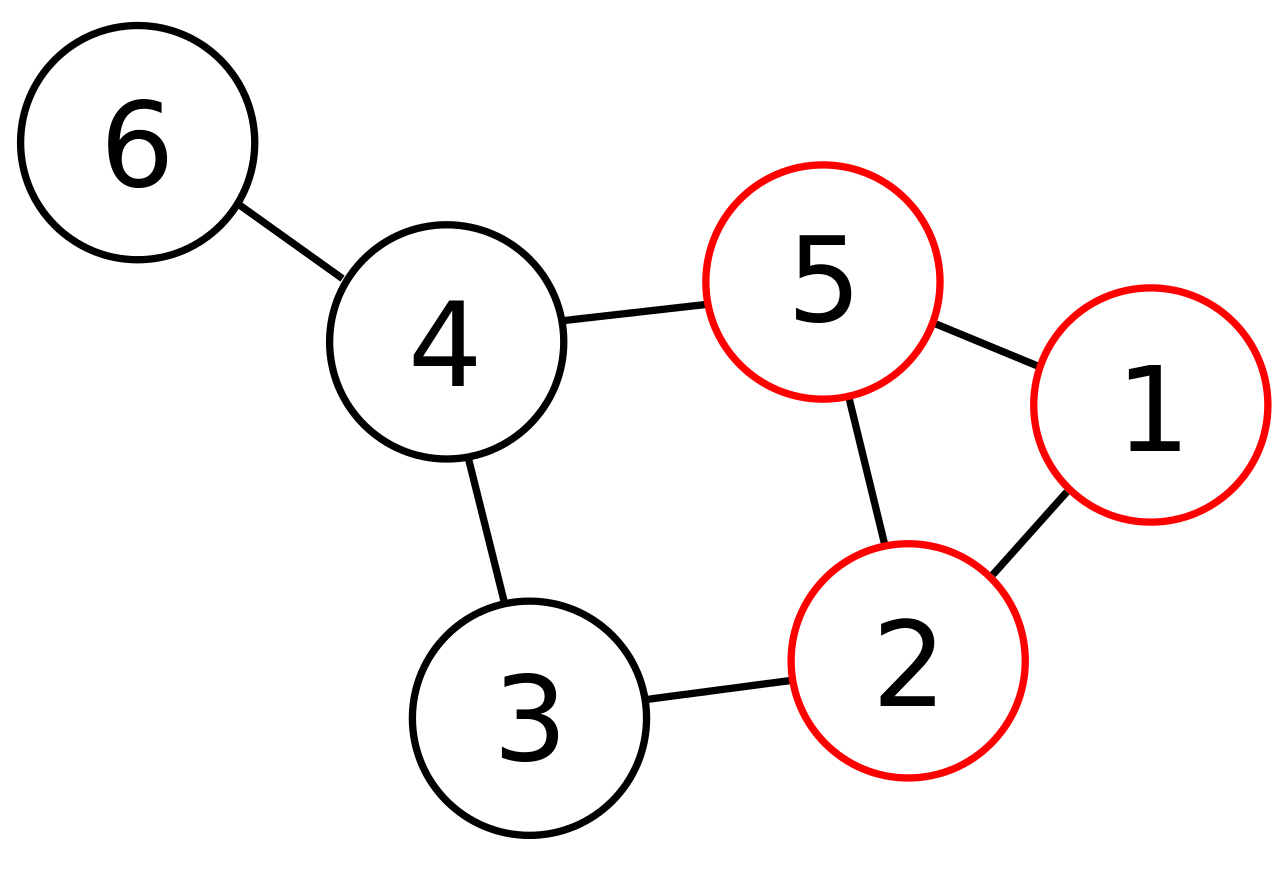
\includegraphics[width=6cm]{figures/clique1.png}
\caption{Ein Graph mit einer Clique der Größe 3.\newline \newline \tiny Quelle: https://de.wikipedia.org/wiki/Clique\_(Graphentheorie)\#/media/File:6n-graf-clique.svg}
\end{figure}
\end{frame}

\begin{frame}{Beispiel}
\begin{figure}
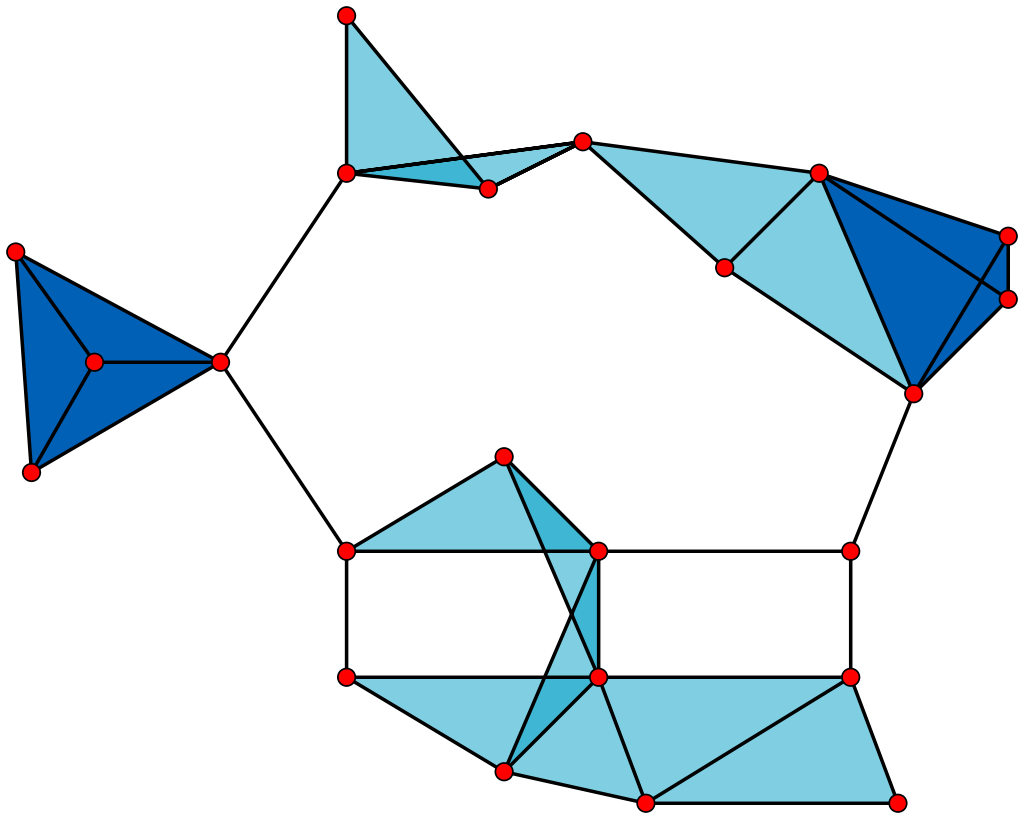
\includegraphics[width=6cm]{figures/clique2.png}
\caption{Ein Graph mit 2 Cliquen der Größe 4.\newline \newline \tiny Quelle: https://en.wikipedia.org/wiki/Clique\_(graph\_theory)\#/media/File:VR\_complex.svg}
\end{figure}
\end{frame}

\begin{frame}{Fragestellungen}
\begin{enumerate}
\item Gibt es eine Clique der Größe k?\\
\textrightarrow Entscheidungsproblem
\newline \pause
\item Berechne das größte k, so dass eine Clique der Größe k vorhanden ist.\\
\textrightarrow Optimale Lösung
\newline \pause
\item Berechne eine Clique mit dem größten k.\\
\textrightarrow Optimierungsproblem
\end{enumerate}
\end{frame}

\subsection{Beweis}
\begin{frame}{CLIQUE Beweis}
Beweis
\end{frame}



\section{Knapsack Problem}
\subsection{Problem}
\begin{frame}{Problem}
Gegeben sind ein Rucksack und \(n\) Objekte mit Gewichten \(g_1,...,g_n \in \mathbb{N}\) sowie eine Gewichtsschranke \(G\).
Zusätzlich seien \(a_1,...,a_n \in \mathbb{N}\) die Nutzenwerte für die Objekte. \cite{wegener}
\pause
\begin{figure}
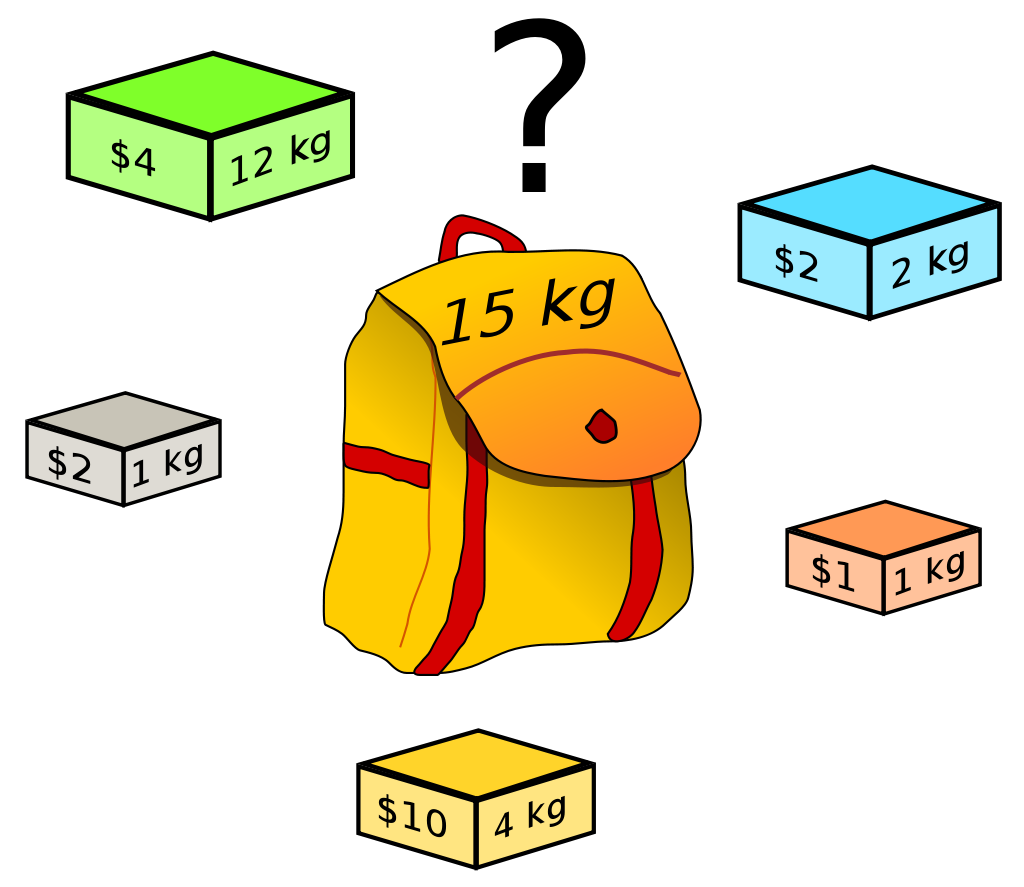
\includegraphics[width=4cm]{figures/knapsack.png}
\caption{Ein zu befüllender Rucksack.\newline \newline \tiny Quelle: https://de.wikipedia.org/wiki/Rucksackproblem\#/media/File:Knapsack.svg}
\end{figure}
\end{frame}

\begin{frame}{Fragestellungen}
\begin{enumerate}
\item Gibt es - unter Beachtung des Limits - eine Beladung mit mindestens diesem Nutzwert?\\
\textrightarrow Entscheidungsproblem
\newline \pause
\item Berechne den größtmöglichen Nutzwert.\\
\textrightarrow Optimale Lösung
\newline \pause
\item Berechne die optimale Beladung.\\
\textrightarrow Optimierungsproblem
\end{enumerate}
\end{frame}

\subsection{Beweis}
\begin{frame}{Beweis}
Beweis
\end{frame}



\section{PARTITION}
\subsection{Problem}
\begin{frame}{PARTITION Problem}
Problem
\end{frame}

\subsection{Beweis}
\begin{frame}{PARTITION Beweis}
Beweis
\end{frame}



\section{BP}
\subsection{Problem}
\begin{frame}{BP Problem}
Problem
\end{frame}

\subsection{Beweis}
\begin{frame}{BP Beweis}
Beweis
\end{frame}



\section{DHC}
\subsection{Problem}
\begin{frame}{DHC Problem}
Problem
\end{frame}

\subsection{Beweis}
\begin{frame}{DHC Beweis}
Beweis
\end{frame}


\section{HC}
\subsection{Problem}
\begin{frame}{HC Problem}
Problem
\end{frame}

\subsection{Beweis}
\begin{frame}{HC Beweis}
Beweis
\end{frame}


\section{TSP}
\subsection{Problem}
\begin{frame}{TSP Problem}
Problem
\end{frame}

\subsection{Beweis}
\begin{frame}{TSP Beweis}
Beweis
\end{frame}

\begin{frame}{Quellen}
\printbibliography
\end{frame}

\end{document}